\documentclass[a4paper]{article}

\usepackage[english]{babel}

\usepackage[utf8]{inputenc}
\usepackage{amsmath}
\usepackage{amsfonts}
\usepackage{cite}
\usepackage{caption}
\usepackage{cases}
\usepackage{graphicx}
\usepackage[colorinlistoftodos]{todonotes}
\usepackage{algorithm}
\usepackage{algpseudocode}
\usepackage{mathtools}
\algnewcommand\algorithmicinput{\textbf{Input:}}
\algnewcommand\INPUT{\item[\algorithmicinput]}
\algnewcommand\algorithmicoutput{\textbf{Output:}}
\algnewcommand\OUTPUT{\item[\algorithmicoutput]}


\usepackage{geometry}
 \geometry{
 a4paper,
 total={210mm,297mm},
 left=20mm,
 right=20mm,
 top=20mm,
 bottom=20mm,
 }
 \usepackage{physics}
 
 
 \usepackage{hyperref}
\hypersetup{
    colorlinks=true,
    linkcolor=blue,
    filecolor=magenta,      
    urlcolor=cyan,
}
 
\urlstyle{same}



\begin{document}



\begin{enumerate}
\item Classification 
	\begin{enumerate}
	\item  K-Nearest Neighbor 
	\item Support Vector Machines
	\item Adaboost 
	\item Iterative Dichotomiser 3
	\item C4.5
	\item Naive Bayes
	\item  Bagging
	\item  Random Forest
	\end{enumerate}
 

	
	
\item Neural Networks
\begin{enumerate}
	\item Perceptron
	\item Back-Propagation
	\item Learning Vector Quantization
	\item Self Organizing Map
	
	
\end{enumerate}	

\item Clustering Algorithms
\begin{enumerate}
   \item Hierarchial Agglomerative Clustering
    \item Hierarchial Division Clustering
\end{enumerate}

\item Regression Algorithms
\begin{enumerate}
   \item Lasso Regression
   \item Logistic Regression
\end{enumerate}

\item Deep Learning Algorithms
\begin{enumerate}
   \item Deep Q-Learning 
\end{enumerate}


\item Other Methods
\begin{enumerate}
   \item Gradient Descent
   \item Gaussian Process
\end{enumerate}

\end{enumerate}


  \begin{algorithm}
 
   \caption{k-Nearest Neighbor  ~ \cite{knearest91} link:{36} }
    \begin{algorithmic}[1]
    \INPUT{X: training data, Y:Class labels of X, $x$: unknown sample}
     \OUTPUT{Class label of unknown sample}
      \Function{Classify}{$X,Y,x$}\
       \For{$i = 1$ to ${m}$}
            \State Compute distance $d{(X_i,x)}$
        \EndFor
        
         \State Compute set $I$ containing indices for the $k$ smallest distances $d{(X_i,x)}$
     
       \State Return majority label $\{Y_i \ \text{where}\ i \in I \}$



 \EndFunction
 


\end{algorithmic}
\end{algorithm}






  \begin{algorithm}
   \caption{Adaboost  ~ \cite{adaboostfirst}}
    \begin{algorithmic}[1]
    \INPUT 
    \Statex Training data $\{(x_i,y_i)_{i=1}^N \ \text{where}\ x_i \in  \mathbb{R}^k \ \text{and} \  y_i \in \{-1,1\} \}$
    \Statex Large number of classifiers denoted by $f_m(x) \in \{-1,1\} $
    \Statex 0-1 loss function $I$ defined as 
 \begin{numcases}{ I(f_m(x,y))=}
  0, & if $ f_m(x_i) = y_i $\\
  1, &  if $ f_m(x_i) \neq y_i $
\end{numcases}
     \OUTPUT{The final classifier}
     
       \For{$i = 1$ to ${N}$}
       \For{$i = 1$ to ${M}$}
            \State Fit weak classifier m to minimize the objective function:
            \State $\epsilon_m =  \frac{\sum_{i=1}^N w_{i}^m I(f_m(x_i)) \neq y_i}{x^2+2x+1} $
            \State where  $I(f_m(x_i) \neq y_i) =1 \  \text{if} \ f_m(x_i) \neq y_i  $ and 0 otherwise
            \State $\alpha_m = \ln \frac{1- \epsilon_m}{\epsilon_m}$
            
        \EndFor
         \For{ all $i$ }
              \State $w_{i}^ {m+1} = w_{i} ^{(m)} e^{\alpha_{mI(f_m(x_i) \neq y_i)}} $ 
         \EndFor 
         
        
        \EndFor
        
        


\end{algorithmic}
\end{algorithm}




  \begin{algorithm}
   \caption{Adaboost ~\cite{adaboostsecond}}
    \begin{algorithmic}[1]
    \INPUT 
    \Statex Training data $\{(x_i,y_i)_{i=1}^N \ \text{where}\ x_i \in  \mathbb{R}^k \ \text{and} \  y_i \in \{-1,1\} \}$
   
     \OUTPUT{Weighted sum that represents the final output of the boosted classifier}
    \State Given Training data $\{(x_i,y_i) \ \text{where}\  \  y_i \in \{-1,1\} \}$
    \State initialize $D_1$ = uniform distribution on training examples
       \For{$t = 1$ to ${T}$}
   
            \State Train weak classifier $h_t \  \text{on}\   \   D_t $
            \State choose $\alpha_t > 0 $
            \State compute new distribution $D_{t+1}$:
             \For{ all $i$ }
              \State multiply $D_t(x)$ by \begin{numcases}{}
  e^{-\alpha_t}, &  ($<1$) $ \text{if}\  \  y_i = h_t(x_i) $\\
   e^{\alpha_t}, & ($>1$) $ \text{if}\  \  y_i \neq h_t(x_i) $
\end{numcases}
\State renormalize
         \EndFor 
         
  \State output final classifier $H_{final(x)} = sign (\sum\alpha_t h_t(x))$
            
        
        
         
        
        \EndFor
        
       


\end{algorithmic}
\end{algorithm}


 \begin{algorithm}
   \caption{Adaboost4 ~\cite{adaboostsecond} Link:23,35,93,95}
    \begin{algorithmic}[1]
     \INPUT 
    \Statex Training data $\{(x_i,y_i)_{i=1}^N \ \text{where}\ x_i \in  \mathbb{R}^k \ \text{and} \  y_i \in \{-1,1\} \}$
   
     \OUTPUT{Weighted sum that represents the final output of the boosted classifier}
     
     \State Set uniform example weights.
     
      \For{each base learner do}
      \State Train base learner with weighted sample.
      \State Test base learner on all data.
      \State Set learner weight with weighted error.
      \State Set example weights based on ensemble predictions.




   
      \EndFor

  
\end{algorithmic}
\end{algorithm}


  \begin{algorithm}
   \caption{Random forest ~\cite{randomforest1} Link:{42} }
    \begin{algorithmic}[1]
    \INPUT{S: training set, F:Features and number of trees in forest $B$}
     \OUTPUT{Constructed tree}
      \Function{RANDOMFOREST}{$S,F$}\
      \State $H \leftarrow  \emptyset $
       \For{$i \in 1,....B$ }
            \State $S^{(i)}\leftarrow \text{A bootstrap sample from} \  S $
            \State $h_i \leftarrow RANDOMIZEDTREELEARN(S^{i},F)$
            \State $H \leftarrow H \bigcup \{h_i\}$
        \EndFor
        \State return $H$
        
        
         



 \EndFunction

  \Function{RANDOMIZEDTREELEARN}{$S,F$}\ 
  \State At each node:
  \State $f \leftarrow \text{a very small subset of} \ F $
  \State Split on best feature in $f$
  \State return The learned tree
   \EndFunction

\end{algorithmic}
\end{algorithm}







  \begin{algorithm}
   \caption{Iterative Dichotomiser 3 ~\cite{id3algo1} Link:{40}}
    \begin{algorithmic}[1]
    \INPUT{$D:\text{Training Data}, \ X: \text{Set of Input  Attributes} $}
     \OUTPUT{A decision tree}
      \Function{ID3}{$D,X$}\
      \State Let $T$ be a new tree 
     \If {all instances in $D$ have the same class $c$}
      \State Label ($T$) = $c$; Return $T$
      \EndIf
      \If {$X= \emptyset\ \text{or no attribute has positive information gain} $}
      \State Label ($T$) = most common class in $D$; Return $T$
      \EndIf
      \State $X \leftarrow \ \text{attribute with highest information gain} $
      \State Label($T$) = $X$
       \For{$\text{each value} \ x \  \text{of} \ X$ }
            \State $D_x \leftarrow \ \text{instances in} \ D \ \text{with} \ X = x $
           \If {$D_x \ \text{is empty}$}
           \State Let $T_x \ \text{be a new tree}$
           \State Label($T_x$) = most common class in $D$
           \Else {\State $T_x$ = ID3($D_x,X-\{x\}$)}
           \EndIf
            \State Add a branch from $T$ to $T_x$ labeled by $x$
        \EndFor
        \State return $T$
         



 \EndFunction

 
\end{algorithmic}
\end{algorithm}


  \begin{algorithm}
   \caption{Perceptron ~\cite{perceptron1} Link:{65}}
    \begin{algorithmic}[1]
    \INPUT{$ProblemSize,InputPatterns,iterations_max,learn_rate$}
     \OUTPUT{$Weights$}
    
       \For{$i = 1$ to ${iterations_{max}}$}
            \State $Pattern_i \leftarrow SelectInputPattern(InputPatterns)$
            \State $Activation_i \leftarrow ActivateNetwork(Pattern_i,Weights)$
            \State $Output_i \leftarrow TransferActivation(Activation_i)$
            \State $UpdateWeights(Pattern_i,Output_i,learn_{rate})$
        \EndFor
        
       
       \State Return $Weights$



 

\end{algorithmic}
\end{algorithm}


  \begin{algorithm}
   \caption{Back-propagation  ~\cite{backpropagation12} Link:17,42}
    \begin{algorithmic}[1]
    \INPUT{$ProblemSize,InputPatterns,iterations_{max},learn_{rate}$}
     \OUTPUT{$Network$}
     \State $Network \leftarrow ConstructNetworkLayers()$
     \State $Network_{weights} \leftarrow InitializeWeights(Network,ProblemSize)$
    
       \For{$i = 1$ to ${iterations_{max}}$}
            \State $Pattern_i \leftarrow SelectInputPattern(InputPatterns)$
            \State $Output_i \leftarrow ForwardPropagate(Pattern_i,Network)$
            \State $BackwardPropagateError(Pattern_i,Output_i,Network)$
            \State $UpdateWeights(Pattern_i,Output_i,Network,learn_{rate})$
        \EndFor
        
       
       \State Return $Network$



 

\end{algorithmic}
\end{algorithm}


\begin{algorithm}
   \caption{Back-propagation2 ~\cite{backpropagation2} }
    \begin{algorithmic}[1]
    \INPUT{
    \Statex Training Set ${x^{(1)}, y^{(1)},,....,(x^{(m)},y^{(m)})}$}
    \OUTPUT{
    \Statex Gradient of the cost function}
    \State $\Delta_{ij}^{(l)} = 0 \text{(for all l,i,j)}$
     \For{$i = 1$ to ${m}$}
     \State Set $a^{(1)} = x ^ {(i)}$
     \State Perform forward propagation to compute $a^{(l)} \  \text{for} \  l =2,3,....L$
     \State Using $y^(i)$, compute $\delta^(L) = a^(L) - y^(i)$
     \State Compute $\delta^(L-1),\delta^(L-2),....\delta^(2) $
    \State $\Delta_{ij}^{(l)} \coloneqq \Delta_{ij}^{(l)} + a_{j}^{(l)}\delta_{i}^{(l+1)} $
      \EndFor
      \State $D_{ij}^{(l)} \coloneqq \frac{1}{m} \Delta_{ij} + \lambda \theta_{ij}^{(l)} \  \text{if}\  j \neq 0 $
      \State $D_{ij}^{(l)} \coloneqq \frac{1}{m} \Delta_{ij} \  \text{if}\  j = 0 $
      \State $\frac{\partial}{\partial\theta_{ij}^{(l)}}J(\theta) = D_{ij}^(l)$ 
      
    
    
    
\end{algorithmic}
\end{algorithm}


  \begin{algorithm}
   \caption{Learning Vector Quantization ~\cite{learningvector3} Link : 50 and 58}
    \begin{algorithmic}[1]
    \INPUT{$ProblemSize,InputPatterns,iterations_{max},CodebookVectors_{num},learn_{rate}$}
     \OUTPUT{$CodebookVectors$}
     \State $CodebookVectors \leftarrow InitializeCodebookVectors(CodebookVectors_{num},ProblemSize) $
     
    
       \For{$i = 1$ to ${iterations_{max}}$}
            \State $Pattern_i \leftarrow SelectInputPattern(InputPatterns)$
            \State $Bmu_i \leftarrow SelectBestMatchingUnit(Pattern_i,CodebookVectors)$
            \For{$Bmu_i ^{attribute} \in Bmu_i $}
            \If{$Bmu_i^{class} \equiv Pattern_i^{class} $}
            \State $Bmu_i^{attribute} \leftarrow Bmu_i^{attribute} + learn_{rate} \times (Pattern_i ^{attribute} - Bmu_i ^{attribute})  $
            \Else { \State $Bmu_i^{attribute} \leftarrow Bmu_i^{attribute} - learn_{rate} \times (Pattern_i ^{attribute} - Bmu_i ^{attribute})  $}
            \EndIf 
            \EndFor  
        \EndFor
        
       
       \State Return $CodebookVectors$



 

\end{algorithmic}
\end{algorithm}



  \begin{algorithm}
   \caption{Self Organizing Map ~\cite{som3} Link:45 }
    \begin{algorithmic}[1]
    \INPUT{$InputPatterns,iterations_{max},learn_{rate},Grid_width,Grid_height$}
     \OUTPUT{$CodebookVectors$}
     \State $CodebookVectors \leftarrow InitializeCodebookVectors(Grid_{width},Grid_{height},InputPatterns) $
     
    
       \For{$i = 1$ to ${iterations_{max}}$}
            \State $Learn_{rate}^i \leftarrow CalculateLearningRate(i,learn_{rate}^{init})$
            \State $neighborhood_{size}^i \leftarrow CalculateNeighborhoodSize(i,neighborhood_{init}^{size})$
            \State $Pattern_i \leftarrow SelectInputPattern(InputPatterns)$
             \State $Bmu_i \leftarrow SelectBestMatchingUnit(Pattern_i,CodebookVectors)$
             \State $Neighborhood \leftarrow Bmu_i$
              \State $Neighborhood \leftarrow  SelectNeighbors(Bmu_i,CodebookVectors,neighborhood_{size}^i)$
            \For{$Vector_i  \in Neighborhood $}
            \For{$Vector_i^{attribute}  \in Vector_i $}
            \State $Vector_i^{attribute} \leftarrow Vector_i^{attribute} + learn_{rate} \times (Pattern_i ^{attribute} - Vector_i ^{attribute})  $
            \EndFor
          
            
            \EndFor
           
        \EndFor
        
       
       \State Return $CodebookVectors$



 

\end{algorithmic}
\end{algorithm}


  \begin{algorithm}
   \caption{Hierarchial Agglomerative Algorithm ~\cite{haa1} Link:24,54}
    \begin{algorithmic}[1]
    \INPUT{\Statex $\langle{V,E,w}\rangle.\text{Weighted graph}$
    \Statex $d_c. \text{Distance measure for two clusters}$}
     \OUTPUT{$\langle{V_T,E_T}\rangle.\text{Cluster hierarchy or dendogram}$}
     \State $C = \{\{v\mid v \in V\}\} $ \Comment{Initial Clustering}
     \State $V_t = \{v_C\mid C \in C\},E_T = \emptyset$ \Comment{Initial Dendogram}
     \While{$\abs{C} > 1$}
     \State $update\_distance\_matrix(C,G,d_c)$
     \State $\{C,C'\} =  \underset{\{C_i,C_j\} \in C : C_i \neq C_j}{argmin} d_c (C_i,C_j)$
     \State $C = (C \backslash \{C,C'\}) \cup \{C \cup C'\}$ \Comment{Merging}
     \State $V_T = V_T \cup \{v_{C,C'}\},E_T = E_T \cup \{\{v_{C,C'} ,v_{C}\},\{v_{C,C'} ,v_{C}\}\}$ \Comment{Dendogram}
     \EndWhile
    
      
        
       
       \State Return $T$



 

\end{algorithmic}
\end{algorithm}


\begin{algorithm}
   \caption{Hierarchial Agglomerative Algorithm 2 ~\cite{.} Link:25,54}
    \begin{algorithmic}[1]
    
    \INPUT{\Statex $\langle{V,E,w}\rangle.\text{Weighted graph}$
    \Statex $d_c. \text{Distance measure for two clusters}$}
     \OUTPUT{$\langle{V_T,E_T}\rangle.\text{Cluster hierarchy or dendogram}$}
       
    \While{More than one cluster remains }
       
    \State Compute the proximity graph if necessary
    
    \State repeat
    
    \State Merge the closest two clusters.
    
    \State Update the proximity matrix to reflect the proximity between the new cluster and the original
clusters.

 \EndWhile



    
    
    

\end{algorithmic}
\end{algorithm}



  \begin{algorithm}
   \caption{Hierarchial Divisive Algorithm ~\cite{hda1}}
    \begin{algorithmic}[1]
    \INPUT{\Statex $\langle{V,E,w}\rangle.\text{Weighted graph}$
    \Statex $d_c. \text{Distance measure for two clusters}$}
     \OUTPUT{$\langle{V_T,E_T}\rangle.\text{Cluster hierarchy or dendogram}$}
     \State $C = \{ V\} $ \Comment{Initial Clustering}
     \State $V_t = \{v_C\mid C \in C\},E_T = \emptyset$ \Comment{Initial Dendogram}
     \While{$\exists{C_x}:(C_x \in C \wedge \abs{C} > 1)$}
     \State $update\_distance\_matrix(C,G,d_c)$
     \State $\{C,C'\} =  \underset{\{C_i,C_j\}  : C_i \cup C_j = C_x   \wedge \  C_i \cap C_j = \emptyset}{argmax} d_c (C_i,C_j)$
     \State $C = (C \backslash \{C,C'\}) \cup \{C \cup C'\}$ \Comment{Merging}
     \State $V_T = V_T \cup \{v_{C,C'}\},E_T = E_T \cup \{\{v_{C,C'} ,v_{C}\},\{v_{C,C'} ,v_{C}\}\}$ \Comment{Dendogram}
     \EndWhile
    
      
        
       
       \State Return $T$



 

\end{algorithmic}
\end{algorithm}


\begin{algorithm}
   \caption{Hierarchial Divisive Algorithm ~\cite{hda1} }
    \begin{algorithmic}[1]
    \INPUT{\Statex $\langle{V,E,w}\rangle.\text{Weighted graph}$
    \Statex $d_c. \text{Distance measure for two clusters}$}
     \OUTPUT{$\langle{V_T,E_T}\rangle.\text{Cluster hierarchy or dendogram}$}
     
        \While{More than one cluster remains }
       
     \State Create a new cluster by breaking the link corresponding to the largest distance (smallest
similarity).

   \EndWhile



\end{algorithmic}
\end{algorithm}

 \begin{algorithm}
 
   \caption{C4.5  ~\cite{c4.5} Link :22,55 }
    \begin{algorithmic}[1]
    \INPUT{
    \Statex $T : \text{Training dataset} $
    \Statex $S : \text{Attributes} $
    }
     \OUTPUT{decision tree $Tree$}
     \Function{C4.5}{$T$}\
      \If {$T \  \text{is} \  NULL $}
      \State return failure
      \EndIf
      
      \If {$S \  \text{is} \  NULL $}
      \State return $Tree \  \text{as a single node with most frequent class label in}\  T$ 
      \EndIf
     
      \If {$\abs{S} = 1 $}
      \State return $Tree \  \text{as a single node}\  S $ 
      \EndIf
      
   \State set $Tree = \{\}$
   
       \For{$a \in S$ }
       \State set $Info(a,T) = 0$  and $SplitInfo(a,T) = 0$
       \State compute $Entropy(a)$
         \For{$v \in values(a,T)$ }
       \State set $T_{a,v}  \text{as the subset of} \  T \  \text{with attribute}\ a = v$  
       \State  $Info(a,T) + = \frac{\abs{T_{a,v}}}{\abs{T_{a}}} Entropy(a)$
       \State $SplitInfo(a,T)+= - \frac{\abs{T_{a,v}}}{\abs{T_{a}}} \log \frac{\abs{T_{a,v}}}{\abs{T_{a}}} $
          \EndFor
          \State $Gain(a,T) = Entropy(a) - Info(a,T)$
          \State  $GainRatio(a,T) = \frac{Gain(a,T)}{SplitInfo(a,T)}$
          \EndFor
       \State set $a_{best} = argmax \{GainRatio(a,T)\}$
       \State $a_{best} \text{into} \  Tree$
        \For{$v \in values(a_{best},T)$ }
       call $C4.5(T_{a,v})$
        \EndFor
        \State return $Tree$
        
  \EndFunction
  

\end{algorithmic}
\end{algorithm}

\begin{algorithm}
 
   \caption{Gradient Descent ~\cite{gradientdescent1} Link : 59 }
    \begin{algorithmic}[1]
    \INPUT{ \Statex $f$
    \Statex starting value $x_{1}$
    \Statex termination tolerances
    }
     \OUTPUT{$x_{maxIters}$}
      
       \For{$i = 1$ to ${maxIters}$}
            \State Compute the search direction $d_t = - \delta f(x_{t})$
            \If {$\abs{d_{T}} < \epsilon_{g} $}
            	\State return "Converged to critical point", output $x_t$
            	\State Find $\alpha_{t}$ so that $f(x_{t}+\alpha_{t}d_{t}) < f(x_t)$
            \EndIf
            
             \If {$\abs{\alpha_{t}d_{T}} < \epsilon_{x} $}
            	\State return "Converged in x", output $x_t$
            	\State Find $\alpha_{t}$ so that $f(x_{t}+\alpha_{t}d_{t}) < f(x_t)$
            	
            \EndIf
            \State Let $x_{t+1} = x_t + \alpha_{t}d_{t}$
            
            
        \EndFor
        
       
       \State Return "Max number of iterations reached", output $x_{maxIters}$
       
       





\end{algorithmic}
\end{algorithm}

 \begin{algorithm}
 
   \caption{Naive Bayes ~\cite{naivebayes1} Link: 9, 56 }
    \begin{algorithmic}[1]
    \INPUT{
    \Statex $C : \text{A fixed set of classes}$
     \Statex $D : \text{ Documents}$
    }
     \OUTPUT{Category(Class) of the Documents}
      \Function{TrainMultinomialNB}{$C,D$}\
       
      \State $V \leftarrow EXTRACTVOCABULARY(D)$
      \State $N \leftarrow COUNTDOCS(D)$
       \For{ each $c \in C$ }
       \State $N_c \leftarrow COUNTDOCSINCLASS(D,c)$
       \State $prior\abs{c} \leftarrow N_{c}/N $
       \State $text_c \leftarrow CONCATENATETEXTOFALLDOCSINCLASS(D,C)$
       \For{ each $t \in V$ }
       \State $condprob\abs{t}\abs{c} \leftarrow  \frac{T_{ct}+1}{\sum_{t'}(T_{ct'+1})}$
      \EndFor
      \EndFor
      \State return $V,prior,condprob$

 \EndFunction
 
 \Function{ApplyMultinomialNB}{$C,D,prior,condprob,d$}\
 \State $W  \leftarrow EXTRACTTOKENSFROMDOC(V,d)$
 
   \For{ each $c \in C$ }
    \State $score\abs{c} \leftarrow  \log \  prior\abs{c}   $
     \For{ each $t \in W$ }
     \State $score\abs{c} += \log condprob\abs{t}\abs{c}$
     
      \EndFor
  \EndFor
 \State return $arg \ max_{c \in C} score\abs{c}$
  \EndFunction
 

\end{algorithmic}
\end{algorithm}


 \begin{algorithm}
 
   \caption{Lasso Regression }
    \begin{algorithmic}[1]
    \INPUT{
    \Statex $ipy:\text{Inner product vector}, ipy_{i} = < y, X._{i} > $
    \Statex $ipx:\text{Inner product matrix}, ipx_{ij} = < X._{i},X._{j} > $
    \Statex $\lambda : \text{Penalty parameter}$
    \Statex $N:\text{Number of samples}$
    
    }
     \OUTPUT{$beta : \text{Regression parameter vector}$}
      \Function{FastLasso}{$ipy,ipx,\lambda , N$}\
      \State $\texttt{stop\_thr}$ \Comment{Threshold for stopping iteration}
      \State $p \leftarrow length(ipy)$
      \State $beta \leftarrow 0 \ \text{with length} \ p$
\State $gc \leftarrow 0 \ \text{with length} \ p$
 \While{$difBeta_{max} \geq \texttt{stop\_thr}  $}
 
 \State $difBeta_{max} \leftarrow  0 $
 
 \For{$j = 1 \leftarrow p $}
 \State $z \leftarrow (ipy\abs{j} - gc\abs{j})/N +beta\abs{j}$
 \State $\texttt{beta\_tmp} \leftarrow max(0,z-\lambda)- max(0,-z-\lambda) $
 \State $difBeta \leftarrow \texttt{beta\_tmp}  - beta\abs{j}$
 \State $difabs \leftarrow abs(difBeta)$
  \If{$difabs > 0$}
  \State $beta\abs{j} \leftarrow \texttt{beta\_tmp} $ 
  \State $gc \leftarrow gc + ipx\abs{j} \times difBeta$
  \State $difBeta_{max} = max(difBeta_{max},difabs)$
  \EndIf
 \EndFor
\EndWhile


 \EndFunction

\end{algorithmic}
\end{algorithm}


  \begin{algorithm}
 
   \caption{Bagging ~\cite{bagging1 } Link:57}
    \begin{algorithmic}[1]
    \INPUT{ \Statex B: the number of bags or base hypotheses
    \Statex L: Base Learning Algorithm}
     \OUTPUT{New Training Sets}
      \Function{Bagging}{$examples,B,L$}\
       \For{$i = 1$ to ${B}$}
            \State $examples_{i} \leftarrow \text{a bootstrap sample of }  examples$
        \EndFor
        
         \State Compute set $I$ containing indices for the $k$ smallest distances $d{(X_i,x)}$
         \State $h_i  \leftarrow \text{apply} L \text{to} examples_{i}$
     
       \State Return $h_{1},h_{2},...h_{B}$



 \EndFunction
 
 \end{algorithmic}
\end{algorithm}

 \begin{algorithm}
 
   \caption{Deep Q-Learning with Experience Replay ~\cite{{DBLP:journals/corr/MnihKSGAWR13}} }
    \begin{algorithmic}[1]
    \INPUT{ \Statex D: data set
    \Statex Q: Action-Value Function}
     \OUTPUT{New Training Sets}
     
       \For{$i = 1$ to ${M}$}
            \State Initialise sequence $s_{1} = \{x_{1}\}$ and preprocessed sequenced $\phi = \phi(s_1)$
             \For{$i = 1$ to ${T}$}
             \State With probability $\epsilon$ select a random action $a_{t}$ otherwise select $a_{t} = max_{a}Q*(\phi(s_{t}).a:\theta)$
             \State Execute action $a_{t}$ in emulator and observe reward  r and image $x_{t+1}$
             \State Set $s_{t+1} = s_{t},a_{t},x_{t+1}$ and preprocess $\phi_{t+1} = \phi(s_{t+1})$
             \State Store transition $(\phi_{t},a_{t},r_{t},\phi_{t+1})$ in $D$
               \State Set $y_{j} = $  \begin{numcases}{}
  r_{j}, &   $ \text{for terminal}\  \  \phi_{j+1} $\\
   r_{j}+\gamma max_{a'}Q(\phi_{j+1,a';\theta}) , &  $ \text{for terminal}\  \phi_{j+1} $
\end{numcases}
\State Perform a gradient descent step on $(y_j - Q (\phi_{j} ,a_{j};\theta))^2$ according to the following equation 
\State $$\Delta_{\theta}L_{i}(\theta_{i}) = \mathbb{E}_{s,a\sim\rho(.);s'\sim \epsilon [(r + \gamma max_{a'}Q(s',a';\theta_{i-1}) - Q (s,a;\theta_{i}))\Delta_{\theta_{i}}Q(s,a;\theta_{i})]  } $$
              \EndFor
        \EndFor
        



 


\end{algorithmic}
\end{algorithm}


 \begin{algorithm}
 
   \caption{PageRank ~\cite{pagerank1
   }  }
    \begin{algorithmic}[1]
    \INPUT{ \Statex $G$: inlink file
    \Statex $iteration$: Number of iteration}
     \OUTPUT{PageRank}
      \Function{PageRank}{$G,iteration$} \
      \State $d \leftarrow 0.85 $ \Comment{damping factor: 0.85}
      \State $oh \leftarrow G $ \Comment{get outlink hash from G}
      \State $ih \leftarrow G $ \Comment{get inlink hash from G}
      \State $N \leftarrow G $ \Comment{get number of pages from G}
       \For{all $p \  \text{in the graph}$}
            \State $opg[p] \leftarrow \frac{1}{N}$
        \EndFor
        \While{$iteration > 0$}
        \State $dp \leftarrow 0 $
        \For{all $p \  \text{that has no out-links }$}
        \State $dp \leftarrow dp + d * \frac{opg[p]}{N} $
        \EndFor
        \For{all $p \  \text{in the graph}$}
        \State $npg[p] \leftarrow dp +  \frac{[1-d]}{N}$
        \For{all $ip \  \text{in}\  ih[p]$}
        \State $npg[p] \leftarrow dp +  \frac{d*opg[ip]}{oh[ip]}$
        \EndFor
        \EndFor
        \State $opg \leftarrow npg$
        \State $iteration \leftarrow iteration -1$
        \EndWhile
        
         


 \EndFunction
 
 \end{algorithmic}
\end{algorithm}


\begin{algorithm}
 \caption{K means    }
    \begin{algorithmic}[1]
     
   \INPUT{
   \Statex $E = \{e_{1},e_{2},....e_{k}\}$
   \Statex $k \text{(number of clusters)}$
   \Statex $MaxIters \text{(limit of iterations)}$}
   \OUTPUT{
   \Statex $C = \{c_{1},c_{2},...c_{k}\}$
   \Statex $L = \{l(e)|e = 1,2,...n\} \ \text{(set of cluster labels of E)}$
   }
   
   \For{each $c_{i} \in C$}
  \State $c_{i} \leftarrow e_{j} \in E \text{(e.g random selection)}$
   
    \EndFor
    
    \For{each $e_{i} \in E$}
    \State $l(e_{i}) \leftarrow argminDistance(e_{i},c_{j})j \in \{1..k\} $
      \EndFor
      \State $changed \leftarrow false$
      \State $iter \leftarrow 0$
    
    \While{$changed = true and iter \leq  = MaxIters $}
    
    \For{$c_{i} \in C$}
    \State $UpdateCluster(c_{i})$
    
     \EndFor
     
     \For{$c_{i} \in E$}
     \State $minDist \leftarrow argminDistance(e_{i},e_{j}) j \in \{1..k\}$
       \If {$minDist \neq l(e_{i})$}
       \State $l(e_i) \leftarrow minDist$
       \State $changed \leftarrow true$
       
       \EndIf
     
    \EndFor
   \State $ iter \texttt{+} \texttt{+}$
      \EndWhile
   

 
 \end{algorithmic}
\end{algorithm}

\begin{algorithm}
 
   \caption{DBSCAN link:{42}  ~\cite{dbscan1
   }  }
    \begin{algorithmic}[1]
    \INPUT{
    \Statex $D$: Data
    \Statex $\epsilon$:Threshold distance
    \Statex $MinPts$ : Minimum number of points required to form a cluster 
    
    }
     \OUTPUT{Clustered Data}
      \Function{DBSCAN}{$D,\epsilon,minPts$}\
      \State $C = 0$
       \For{$\text{each point}\ P \text{in dataset} D$}
        \If {$P$ is visited}
        \State continue next point
      
        \EndIf
            \State mark P as visited
            \State $NeighborPts = regionQuery(P,\epsilon)$
            \If {$sizeof(NeighborPts) < MinPts$ }
            \State mark P as NOISE
            \Else{
            \State $C = \text{next cluster}$
            \State $expandCluster(P,NeighborPts,C,\epsilon, MinPts)$
            }            
            \EndIf
        \EndFor
        
      



 \EndFunction
 
    \Function{expandCluster}{$P,NeighborPts,C,\epsilon,MinPts$}\
    \State add P to Cluster C
    \For{$\text{each point} \ P' in NeighborPts$}
    \If{$P' \ \text{is not visited}$}
     \State mark $P'$ as visited
     \State $NeighborPts' = regionQuery(P', eps)$
      \If {$sizeof(NeighborPts) >= MinPts$ }
      \State  $NeighborPts = NeighborPts \ \text{joined with}\ NeighborPts'$
     \EndIf
    \EndIf
     \If{$P' \ \text{is not yet member of any cluster}$}
     \State add $P'$ to cluster $C$
     \EndIf
    \EndFor

 \EndFunction

  \Function{regionQuery}{$P,\epsilon$}\
  \State return all points within $P's \ \epsilon \ neighborhood$
   \EndFunction
\end{algorithmic}
\end{algorithm}
 

\begin{algorithm}
  \caption{Principle Component Analysis ~\cite{.
   } }
  
\begin{algorithmic}[1]
 \INPUT
 \Statex $x_{1},.....x_{n} \text{d length vector k}$
 \OUTPUT{Transform matrix R}
 \State $X \leftarrow n \times d \ \text{data matrix with } x_{i} \  \text{in each row}$
\State  $x \leftarrow  \frac{1}{n} \sum_{i = 1}^{n} x_{i}$
\State $X \leftarrow \text{subtract x from each row} \  x_{i} in X $
\State $COV \leftarrow \frac{1}{n-1}X^{T} \times X \text{Compute eigenvalue} \  e_{1},....,e_{d} \  \text{of COV, and sort them }$
\State Compute matrix $V$ which satisfy $V^{-1} \times COV \times V = D$ , $D$ is the diagonal matrix of eigenvalue of COV
\State $R \leftarrow \text{the first}\  k \ \text{column of} \ V$

\end{algorithmic}
\end{algorithm}


  \begin{algorithm}
   \caption{Logistic Regression  ~\cite{logistic1
   } }
    \begin{algorithmic}[1]
    \INPUT 
    \Statex Training data of the form $\{(x_{1},1),(x_{2},0),..\}$
    \Statex  $x$: unknown sample
     \OUTPUT{The output is a probability that the given input point belongs to a certain class}
    \State $0 \leftarrow \beta$
 \State Compute y by setting its elements to
   \begin{numcases}{ y =}
  1, & if $g_{i} = 1 $\\
  0, &  if $g_{i} = 2 $
\end{numcases}
 i = 1,2,..N
 \State Compute p by setting its elements to
 $$p(x_{i},\beta) = \frac{e^{\beta^{T}x_{i}}}{1+ e^{\beta^{T}x_{i}}} $$   i = 1,2,..N
 
\State Compute the diagonal matrix W. The ith diagonal element is  $p(x_{i},\beta)(1-p(x_{i};\beta))$
    
\State $z \leftarrow X\beta + W ^{-1}(y - p) $

\State $\beta \leftarrow (X^{T}WX)^{-1}X^{T}Wz$

\State If the stopping criteria,stop;otherwise go back to step 3
    
     
       
        


\end{algorithmic}
\end{algorithm}



 \begin{algorithm}
   \caption{Gaussian Process ~\cite{gaussian1
   }}
    \begin{algorithmic}[1]
  \INPUT 
 \Statex $X =  \begin{bmatrix}
 	x_{1}^T\\
 	\hdotsfor{1}\\
    x_{n}^T 
 \end{bmatrix} \in 	\mathbb{R}^{ n \times D} , \text{m training inputs}
 $
 
  \Statex $y =  \begin{bmatrix}
 	y_{1}^T\\
 	\hdotsfor{1}\\
    y_{n}^T 
 \end{bmatrix} \in 	\mathbb{R}^{ n}
 $ 
 \Statex $k(.,.): \mathbb{R}^ {D \times D}$
 \Statex $x_{*} \text{test input}$
 \Statex $\sigma^{2} \text{noise level on the observations}$
 $$[y(x) = f(x) + \epsilon , \epsilon \sim N (0, \sigma^{2})] $$
\OUTPUT{
\Statex ${f_{*}}$
\Statex $cov(f_{*})$
}

\State $K \in \mathbb{R}^{n \times n} \text{Gram matrix}. K_{ij} = k(x_{i}, x_{j})
$

$$k(x_{*}) = k_{*} = k(X,x_{*}) = \begin{bmatrix}
	k{(x_{1},x_{*})}\\
 	\hdotsfor{1}\\
    k{(x_{n},x_{*})}
 \end{bmatrix} \in \mathbb{R}
 $$
 
 \State $\alpha = (K + \sigma_{2}\mathbb{I}_{n})^{-1}y$
 \State $f_{*} = k_{*}^{T}\alpha \in \mathbb{R} $
 
 \State $cov(f_{*}) = k(x_{*},x_{*}) - k_{*}^T[K+\sigma_{2}\mathbb{I}n]^{-1}k_{*}$



\end{algorithmic}
\end{algorithm}


\begin{algorithm}
 \caption{Support Vector Machines ~\cite{svm1
   }}
    \begin{algorithmic}
    \INPUT {
    \Statex Set of N input-output pairs $\{x,y\}^{N_1}$ x: input vectors of the same dimension and y : set of output target labels $ y_i = \{0,1\} $
    }
 \begin{sloppypar}
 
  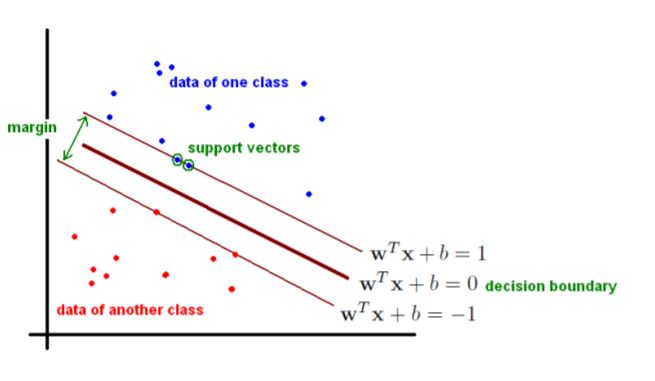
\includegraphics[width=\linewidth]{svm.jpg}
  
  \label{fig:svm1}


\end{sloppypar}
 
 \section{ Simple case : linearly-separable data,binary classification}
 
\paragraph{}
 Goal:we want to find the hyperplane(i.e. decision boundary)linearly
 separating our classes. Our boundary will have the equation: $\textbf{w}^ \textbf{T}\textbf{x}+ \textbf{b} = 0$
 
 \paragraph{}
 Anything above the decision boundary should have label 1 i.e., $\textbf{w}^\textbf{T}\textbf {x}_{i} + b  > 0 $ will have corresponding $y_{i} = 1$
 
\paragraph{}
Similarly, anything below the decision boundary should have label -1 i.e.
 $\textbf{w}^\textbf{T}\textbf {x}_{i} + b  < 0 $ will have corresponding $y_{i} = - 1$

\paragraph{}
The reason for this labeling scheme is that it lets us condense for the decision function to 
$$f(x) = sign(\textbf{w}^\textbf{T} + b )$$ since $f(x) = +1 $ for all x above the boundary , and $f(x) = -1$ for all x below the boundary.

\paragraph{}
Thus, we can figure out if an instance has been classified properly by checking that $y(\textbf{w}^\textbf{T} + b ) \geq 1 $ (which will be the case as long as either both $y, \textbf{w}^\textbf{T} + b > 0 \  \text{or else} \  y,   \textbf{w}^\textbf{T} + b < 0 $)

\paragraph{}
You'll notice that we will now have some space between our decision boundary and the nearest data points of either class. Thus,let's rescale the data such that anything on or above the boundary $\textbf{w}^\textbf{T}\textbf {x} + b = 1 $ is of one class(with label 1), and anything on or below the boundary $\textbf{w}^\textbf{T}\textbf {x} + b = -1 $ is of another class (with label -1)

\paragraph{}
What is the distance between these newly added boundaries?
\paragraph{}
First note that the two lines are parallel,and thus share their parameters $w,b$.Pick an arbitary point $x_{1}$ to lie on line $ \textbf{w}^\textbf{T}\textbf {x} + b = -1 $. Then the closest point on line $ \textbf{w}^\textbf{T}\textbf {x} + b = 1 $ is the point $\textbf{x}_{2} = \textbf{x}_{1} + \lambda\textbf{w} $(since the closest point will always lie on the perpendicular;recall that the vector $\textbf{w}$ is perpendicular to both lines). Using this formulation, $\lambda\textbf{w}$ will be the line segment segment connecting $\textbf{x}_{1}$ and $\textbf{x}_{2}$ , and thus, $\lambda\ \|\textbf{w}\|$, the distance between $\textbf{x}_{1}$ and $\textbf{x}_{2}$ is the shortest distance between the two lines/boundaries.




 \algstore{myalg}

\end{algorithmic}
\end{algorithm}

\clearpage

\begin{algorithm}
  \ContinuedFloat
  \caption{Support Vector Machines (continued)}
  \begin{algorithmic}
      \algrestore{myalg}
      \State
Solving for $\lambda$ : $\textbf{w}^\textbf{T}\textbf{x}_{2} + b = 1$ where $\textbf{x}_{2} = \textbf{x}_{1} +   \lambda\textbf{w} $ \newline $\textbf{w}^\textbf{T}(\textbf{x}_{1} \lambda\textbf{w}) +  b = 1$  
$\textbf{w}^\textbf{T}(\textbf{x}_{1} \lambda\textbf{w}) +  b = 1$ \newline $\textbf{w}^\textbf{T}\textbf{x}_{1} + b + \lambda\textbf{w}^\textbf{T}\textbf{w} = 1 $ where $\textbf{w}^\textbf{T}\textbf{x}_{1} + b = -1 $  \newline $-1 + \lambda\textbf{w}^\textbf{T}\textbf{w} = 1$ \newline $\lambda\textbf{w}^\textbf{T}\textbf{w} = 2$
\newline $\lambda = \frac{2}{\textbf{w}^\textbf{T}\textbf{w}}  = \frac{2}{\|\textbf{w}\|^2}$ \newline And, so the distance $\lambda\|w\| is   \frac{2}{\|\textbf{w}\|^2}\|w\| = \frac{2}{\|w\|} = \frac{2}{\sqrt{\textbf{w}^\textbf{T}\textbf{w}}}$



\paragraph{}
It's intuitive that we would want to maximize the distance between the two boundaries demarcating the classes(Why?We want to be as sure that we are not making classification mistakes and thus we want our data points from the two classes to lie as far away from each other as possible).This distance is called the margin,so went to obtain the maximal margin.

      
   \paragraph{}
Thus, we want to maximize $\frac{2}{\sqrt{\textbf{w}^\textbf{T}\textbf{w}}}$, which is equivalent to minimizing $\frac{\sqrt{\textbf{w}^\textbf{T}\textbf{w}}}{2}$ which is in turn equivalent to minimizing $\frac{\textbf{w}^\textbf{T}\textbf{w}}{2}$(since square root is a monotonic function)
      
   \paragraph{}
This quadratic programming problem is expressed as :\newline
 $min_{w,b}\frac{\textbf{w}^\textbf{T}\textbf{w}}{2}$ \newline
 subject to : $y_{i}(\textbf{w}^{T}\textbf{x} + b) \geq 1 (\forall \ \text{data points} \ \textbf{x}_{i} )$
   
     
\section{Soft-margin extension}

\paragraph{}
Consider the case that your data isn't linearly separable.For instance,
maybe you aren’t guaranteed that all your data points are correctly labelled, so you want to allow some data points of one class to appear on the other side of
the boundary.


\paragraph{}
We can introduce $slack variables \text{an}-\epsilon_{i} \geq 0$. Our quadratic programming problem becomes:\newline
$min_{\textbf{w},b,\epsilon} \frac{\textbf{w}^\textbf{T}\textbf{w}}{2}+ C\sum_{i}\epsilon_{i}$\newline
subject to : $y_{i}(\textbf{w}^\textbf{T}\textbf{x}_{i}+ b) \geq 1 -\epsilon$
 
\section{Nonlinear decision boundary}

\paragraph{}
Mapping your data vectors, $x_{i}$,into a higher-dimension(even infinite) feature space may make them linearly separable in  that space (whereas they may not be linearly separable in the original space). The formation of the quadratic programmatic problem is as above,but with all $\textbf{x}_{i}$ replaced with $\phi(\textbf{x}_{i}),\text{where} \ \phi $provides the higher-dimensional mapping.So we have the standard SVM formulation: \newline
$min_{\textbf{w},b,\epsilon}\frac{\textbf{w}^T\textbf{w}}{2}$\newline
subject to : $y_{i}(\textbf{w}^T\phi(\textbf{x}_{i}) + b ) \geq 1 - \epsilon \text{and} \ \epsilon_{i} \geq 0 (\forall \  \text{data points} \  \textbf{x}_{i})$

\section{Reformulating as a Lagrangian}
\paragraph{}
We can introduce Lagrange multipliers to represent the condition:\newline
$y_{i}(\textbf{w}^T\phi(\textbf{x}_{i} + b ))$ must be as close to 1 as possible.  This condition is captured by: $max_{ai \geq 0}\alpha_{i}[1-y_{i}(\textbf{w}^T\phi(\textbf{x}_{i} + b ))]$ This ensures that when $y_{i}(\textbf{w}^T\phi(\textbf{x}_{i} + b )) \geq 1$, the expression above is maximal when $\alpha_{i} = 0$(since [1- $y_{i}(\textbf{w}^T\phi(\textbf{x}_{i} + b )$] ends up being negative). Otherwise, $y_{i}(\textbf{w}^T\phi(\textbf{x}_{i} + b )) < 1 $, so $[1- y_{i}(\textbf{w}^T\phi(\textbf{x}_{i} + b ))]$ is a positive value, and the expression is maximal when $a_{i} \rightarrow \infty$. This has the effect of penalizing any misclassified data points, while assigning $0$ penalty to properly classified instances.

\paragraph{}
We thus have the following formulation: \newline
$min_{w,b}[\frac{\textbf{w}^T\textbf{w}}{2} + \sum_{i}max_{\alpha \geq 0} \alpha_{i}[1-\textbf{w}^T\phi(\textbf{x}_{i} + b )]]$ \newline
To allow for slack(soft-margin), preventing the $\alpha$ variables from going to $\infty$, we can impose constraints on the Lagrange multipliers to lie within: $0 \leq \alpha_{i} \leq C$.
We can define the dual problem by interchanging the max and min as follows (i.e minimize after fixing alpha): \newline
$max_{alpha \geq zero}[min_{w,b}J(\textbf{w},b;\alpha)] \text{where} \ = \frac{\textbf{w}^T\textbf{w}}{2}+ \sum_{i}\alpha_{i}[1 - y_{i}(\textbf{w}^T\phi(x_{i}) + b)]$


 \algstore{myalg}

   
 \end{algorithmic}
\end{algorithm}
 
 \begin{algorithm}
  \ContinuedFloat
  \caption{Support Vector Machines (continued)}
  \begin{algorithmic}
      \algrestore{myalg}
      \State
 \paragraph{}
Since, we're solving an optimization problem, we set $\frac{\partial  J}{\partial \textbf{w}} = 0 $ and discover that the optimal setting of $\textbf{w}$ is $\sum_{i}\alpha_{i}y_{i}\phi(x_{i}) $,while seeting $\frac{\partial  J}{\partial \textbf{b}} = 0 $ yields the constraint $\sum_{i}\alpha_{i}y_{i} = 0$
      
\paragraph{}
Thus, after substituting and simplifying,we get: \newline
$min_{w,b}J(\textbf{w},b,\alpha) = \sum_{i}\alpha_{i}\alpha_{j}y_{i}y_{j}\phi(\textbf{x}_{i})^T \phi(\textbf{x}_{j}) $
And thus our dual is: \newline
$max_{\alpha \geq 0}[\sum_{i}\alpha_{i} - \frac{1}{2} \sum_{i,j}\alpha_{j}y_{i}y_{j}\phi(\textbf{x}_{i})^T \phi(\textbf{x}_{j})]$\newline Subject to: $\sum_{i}\alpha_{i}y_{i} = 0  \ \text{and} \ 0 \leq \alpha_{i} \leq C$   
      
      
\section{Kernel trick}
\paragraph{}

Because we're working in a higher-dimension space(and potentially even an infinite-dimensional space),calculating $\phi(\textbf{x}_{i})^T \phi(\textbf{x}_{j})$ may be intractable.However, it turns out there are special $kernel$ functions that operate on the lower dimension vectors $\textbf{x}_{i}$ and $\textbf{x}_{j}$ to produce a value equivalent to the dot-product of the higher dimensional vectors.
For instance, consider the function $\phi \mathpunct{:} \mathbb{R}^3 \longmapsto \mathbb{R}^{10} ,where: $
$\phi(x) = (1,\sqrt{2}x^{(1)} ,\sqrt{2}x^{(2)}, \sqrt{2}x^{(3)} ,[\textbf{x}^{(1)}]^2 ,[\textbf{x}^{(2)}]^2, [\textbf{x}^{(3)}]^2, \sqrt{2}x^{(1)(2)} ,\sqrt{2}x^{(1)(3)} ,\sqrt{2}x^{(2)(3)} )  $
Instead, we have the the kernel trick, which tells us that $K(\textbf{x}_{i},\textbf{x}_{j} ) = (1+\textbf{x}_{i}^T\textbf{x}_{j})^2 = \phi(\textbf{x}_{i})^T\phi(\textbf{x}_{j})$ for the given $\phi$. Thus, we can simplify our calculations.
Re-writing the dual in terms of the kernel yields:
$max_{\alpha \geq 0}[\sum_{i}\alpha_{i} - \frac{1}{2}\sum_{i,j}\alpha_{i}\alpha_{j}y_{i}y_{j}]$


      
      \section{Decision function}
To classify a novel instance $\textbf{x}$ once you've learned the optimal $\alpha_{i}$ parameters, all you have to do is calculate $f(\textbf{x}) = sign(\textbf{w}^T\textbf{x}+b) = \sum_{i}\alpha_{i}y_{i}\phi(\textbf{x}_{i}\  \text{and using the kernel trick})$. Note that $\alpha_{i}$ is only non-zero for instances $\phi(\textbf{x}_{i})$ on or near the boundary-those are called the $support vector $ since they alone specify the decision boundary. We can toss out the other data points once training is complete. Thus, we only sum over the $x_{i}$ which constitute the support vectors.
  \end{algorithmic}
\end{algorithm} 
      
 \newpage



\bibliographystyle{apalike}
\bibliography{Bibiliography}


\end{document}



